\section{Durchführung}
\label{sec:Durchführung}
\subsection{Versuchsaufbau}
Das Geiger-Müller-Zählrohr wird an eine Spannungsquelle angeschlossen.
Vor das Zählrohr wird zur Messung eine $\beta$-Teilchen Quelle gestellt.

\subsection{Charakteristik des Geiger-Müller-Zählrohr}
\label{subsec:charak}
Zur Ermittlung der Charakteristik wird nun die Zählrate des Geiger-Müller-Zählrohrs gemessen.
Dafür wird die Spannung am Zählrohr zunächst auf $\SI{320}{\V}$ gestellt.
Nun werden die Anschläge des Zählrohrs in einem Zeitintervall von $t=60\si{\second}$ gemessen.
Der Zeitintervall ist dabei so gewählt, dass die Impulse pro Zeitintervall im Bereich von $N=10000 \, \text{Imp}$ liegen.
Dies geschieht um die Unsicherheit durch die Totzeit möglichst im Bereich von $1\%$ zu halten.
Nach der Messung wird die Spannung um $\Delta U = 10\si{\V}$ erhöht und die Anschläge werden erneut gemessen.
Der Prozess, wird bis zu einer Spannung von $700\si{\V}$ wiederholt.
\FloatBarrier
\subsection{Totzeitbestimmung}
\label{subsec:tot}
Die Totzeit wird mit der Zwei-Quellen-Methode ermittelt.
Dafür wird zunächst der Versuchsaufbau, wie in Abbildung \ref{fig:aufbau} dargestellt, umgebaut.
Wie in der Abbildung zu sehen ist, muss um $N_1$ zu messen die Teilchenquelle zuerst in die dafür vorgesehene Halterung gebracht werden.
Nach einer Integrationszeit von $120\si{\second}$ wird die Anzahl der Impulse festgehalten.
Die zweite Teilchenquelle wird zusätzlich zur ersten in die dafür vorgesehende Halterung gebracht und die Messung wird gestartet.
Auch diese wird mit einer Integrationszeit von $120 \si{\second}$ durchgeführt.
Durch die Messung wird der Wert $N_{1+2}$ erhalten.
Zuletzt wird der Wert $N_2$ gemessen.
Dafür wird die Teilchenquelle welche zur Messung von $N_1$ genutzt wurde wieder entnommen.
Auch hier beträgt die Integrationszeit $120\si{\second}$.

\begin{figure}
    \centering
    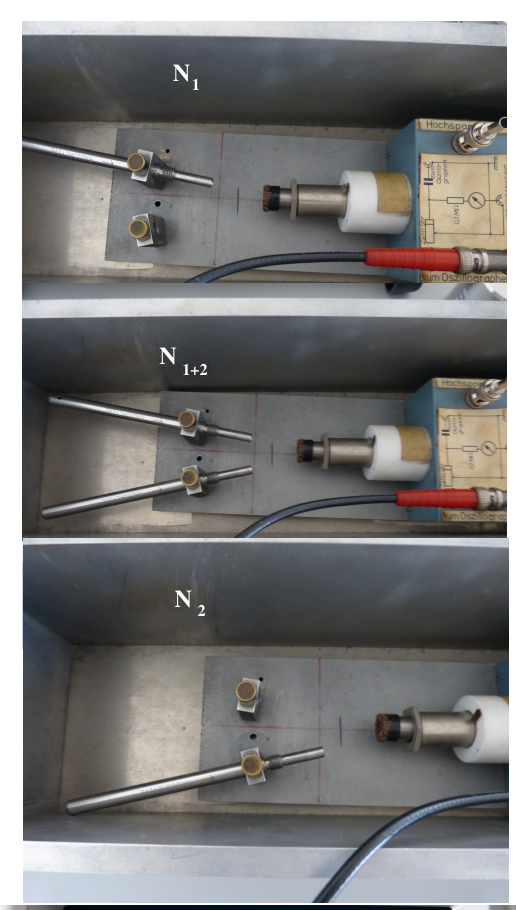
\includegraphics[width=0.4\textwidth]{content/data/aufbau.png}
    \caption{Der Versuchsaufbau für die Zwei-Quellen-Methode, Abbildung entnommen aus \cite{anleitung}.}
    \label{fig:aufbau}
\end{figure}
\FloatBarrier
\subsection{Freigesetzte Ladung pro eingefallenem Teilchen}
Während der Messung, die in \ref{subsec:charak} beschrieben wurde, wurde neben den Impulsen, auch der Zählerstrom $I$ des Zählrohrs notiert.
Dieser wird in dem Bereich \ref{sec:Auswertung} genutzt um den gesuchten Wert $Z$, die Anzahl der pro Teilchen freigesetzten Ladungen, zu berechnen.